\section{Theoretischer Hintergrund}
\label{sec:theory}

Internet of Things (IoT) ist ein Gebiet, welches dem Alltag viele Vorteile bringt. Durch die Möglichkeit
Geräte aus dem Alltag mit dem Internet zu verbinden, birgt IoT aber auch Sicherheitslücken die besagte Geräte sehr Gefährlich
werden lässt. Um dem entgegen zu wirken soll sich die Dissertation im Gebiet der Malwareforschung befinden. Im speziellen soll es dabei um 
die Erkennung von Botnetzen gehen, welche Angriffe über IoT-Geräte ausführen. \\ Ein Botnetz ist der Zusammenschluss von Hosts, auch Bots oder Zombies genannt, gesteuert von einem Angreifer, 
auch Botmaster genannt in einem Overlay-Netzwerk \cite{Xing2021SurveyOB}. Die Botnetze nutzen Zero-day Schwachstellen, Peer-2-Peer Netze, Phishing Angriffe, Anonyme Netzwerke,
Blockchain Netzwerke und Stromnetze zur Verbreitung für ihre Verwendungszwecke \cite{DBLP:conf/cycon/CasenoveM14,DBLP:conf/esorics/KurtECAU20}. Auf Basis der Architektur 
des Botnetzes findet zu jeder Zeit ein Kommunikations- und Kontrollprozess mit dem Command und Control (C\&C)-Server statt. Der C\&C-Server gibt den Bots Befehle die 
diese dann durchführen \cite{SCHILLER200729} zum Beispiel, über das Internet Relay Chat (IRC)-Protokoll. Der Botmaster kann aber auch ohne den C\&C-Server Nachrichten an die Bots leiten, wie
später die verschiedenen Architekturen zeigen. \\ Botnetze durchlaufen drei Phasen wie Wazzan et al. 
\cite{Wazzan2021InternetOT} beschreiben, scannen, ausbreiten und angreifen. Während der Scan-Phase sucht ein Bot nach vulnerablen IoT-Geräten und 
infiziert das Gerät entweder durch brute force Methoden oder durch Ausnutzen einer Schwachstelle.
In der Ausbreitungs-Phase ist eine lauffähige Version des Bots installiert und auf Basis der Architektur des infizierten Geräts ausgeführt.
Um auf dem Gerät Malware zu verhindern die nicht vom Bot selbst ausgeführt wird, stoppt der Bot andere Prozesse um Ports für sich selbst zu blocken. 
Daraufhin rekrutiert das bösartige Programm weitere Bots um das Botnetz so schnell wie möglich zu erweitern. In der Angriffs-Phase führt das Botnetz Angriffe wie Distributed Denial of 
Service (DDoS), krypto mining und spam Angriffe aus. Die erläuterten Phasen arbeiten auch Studien wie \cite{10.1007/978-3-030-33229-7_21, Alzahrani2020,DBLP:journals/computer/VlajicZ18,NGUYEN2020128} 
aus. Dennoch lassen sich die drei Phasen in weitere Phasen aufteilen und können je nach Verwendungszweck des Botnetzes varriieren. Botnetze können nach verschiedenen Architekturen aufgebaut sein: 
zentralisiert, Peer-to-Peer(P2P) Architekturen \cite{DBLP:journals/fi/VuSEBD21} und hybride Architekturen \cite{DBLP:conf/ecai2/ApostolTP22}. Bei zentralen Botnetzen kommuniziert der Botmaster
über einen zentralen C\&C-Server mit den Bots, während bei den dezentralen P2P Architekturen der Botmaster die Befehle über das gesamte P2P-Overlay-Netzwerk verteilt und hybride Architekturen kombinieren 
die beiden vorangegangen Architekturen. IoT Botnetze fallen dabei nicht in eine der drei Architekturen. Für IoT Botnetze sind alle Architekturen möglich \cite{DBLP:conf/csndsp/McNultyV22}. \\ Nach der Erläuterung 
wie Botnetze funktionieren und welche es gibt, ist nun zu klären, wie der Prozess eines Botnetzes erkennbar ist um IoT-Geräte entsprechend zu schützen. Nach Xing et al. \cite{Xing2021SurveyOB} kann die Botnetz 
Erkennung in Honeypot Analyse, Signaturen aus der Kommunikation und abnormales Verhalten klassifiziert werden. Wie Abbildung \ref{fig:bot_det_met} zeigt, unterteilen diese Klassifikationen Methoden zur Erkennung. 

\begin{figure}[h!]
    \centering
    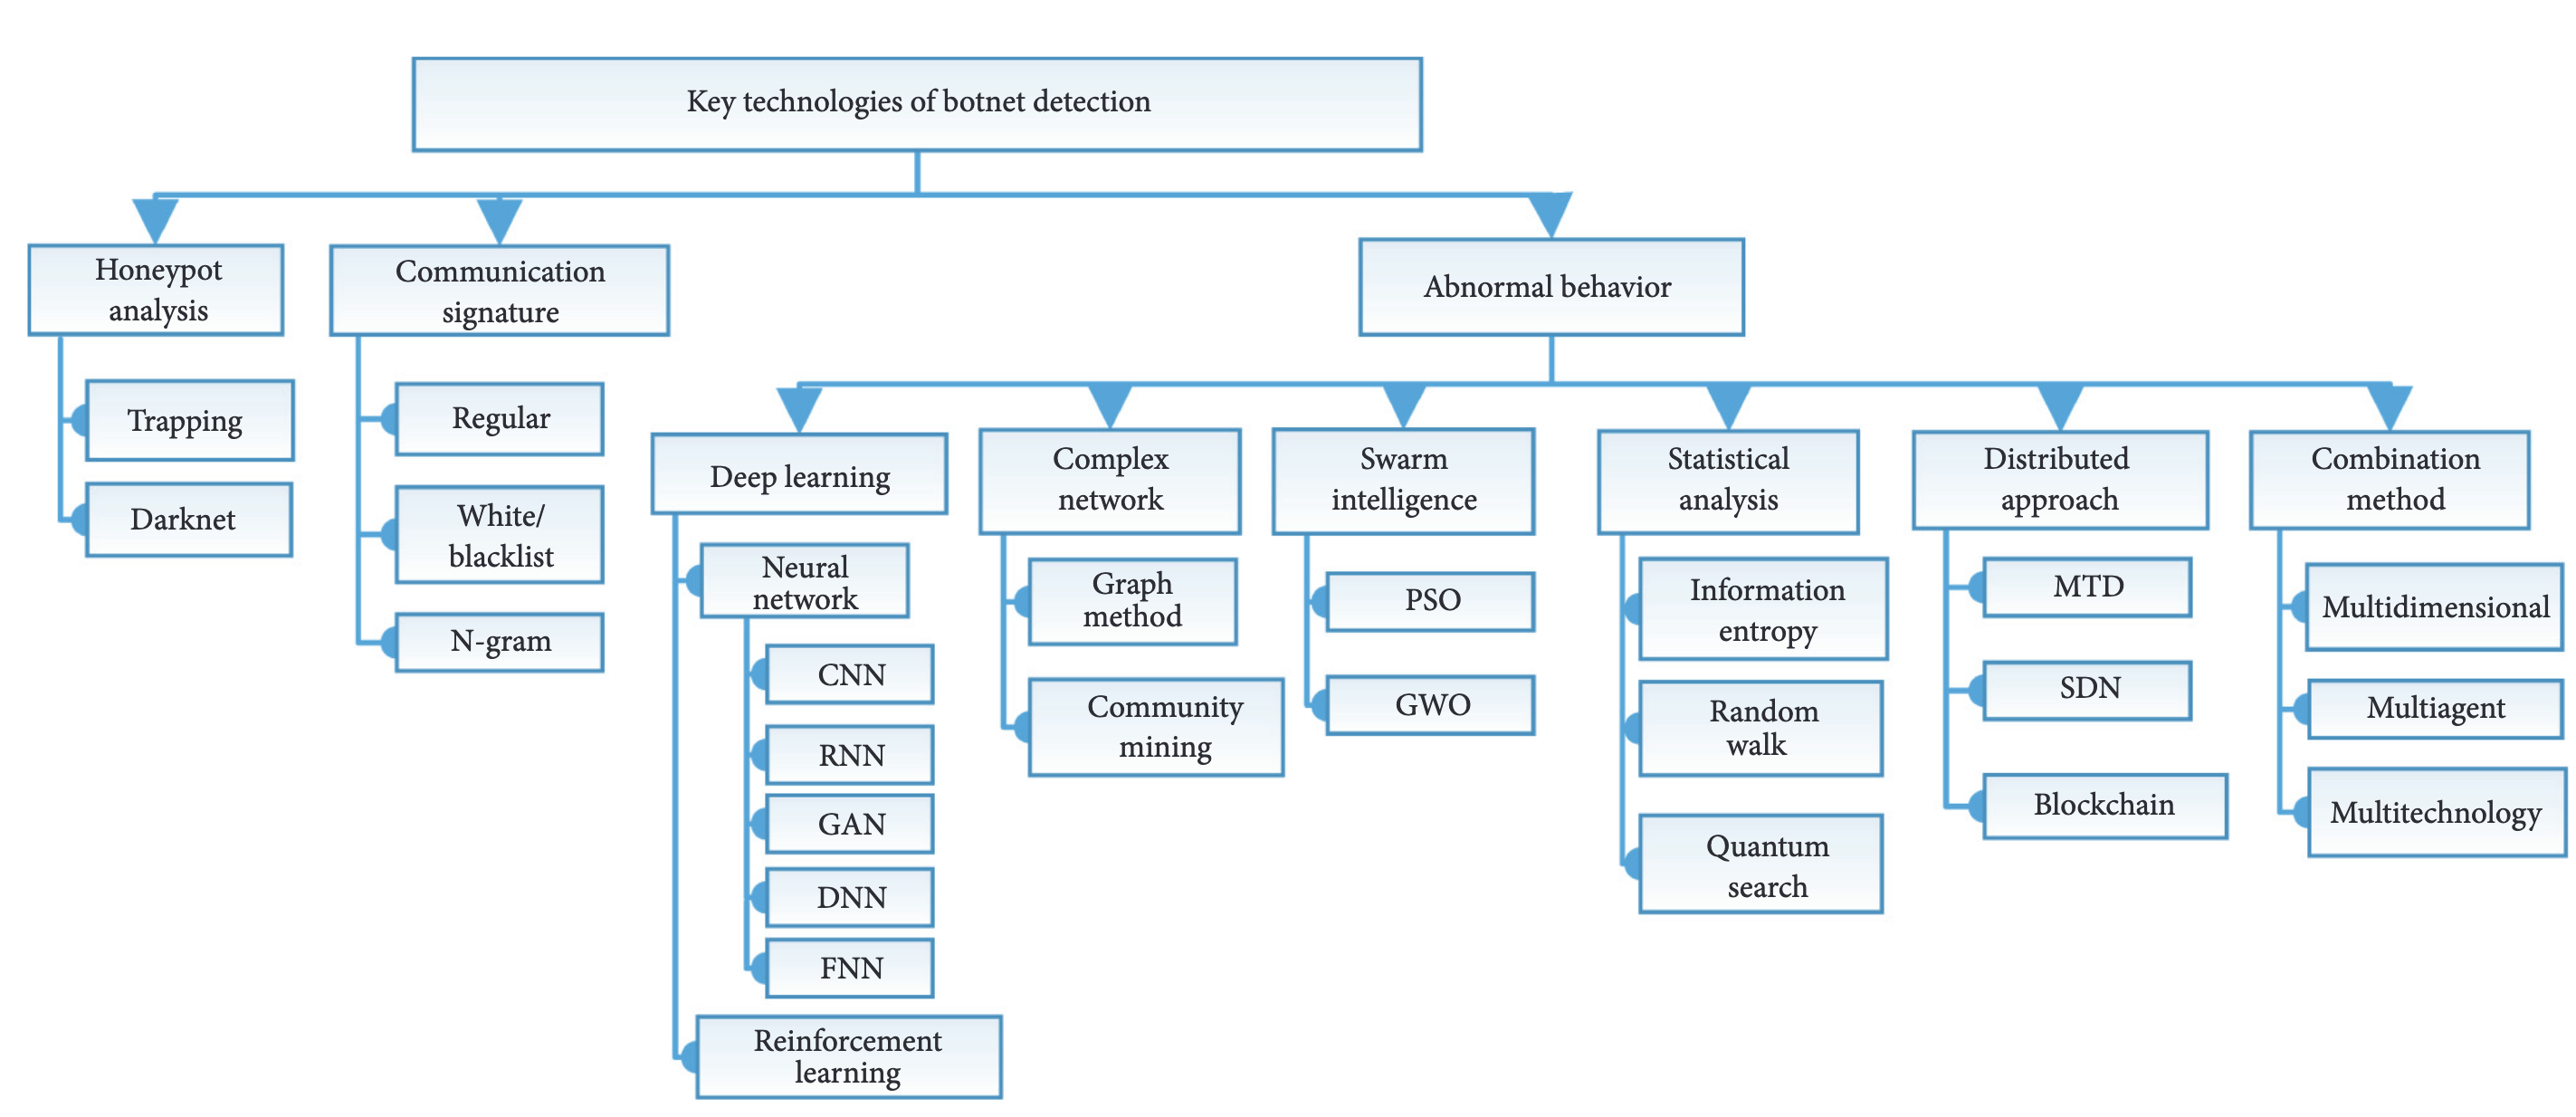
\includegraphics[scale=0.314]{./pictures/botnet_detection_methods.png}
    \caption{Klassifizierte Erkennungsmethoden von Botnetzen (übernommen von \cite{Xing2021SurveyOB}).}
    \label{fig:bot_det_met}
\end{figure}

Die \textit{Honeypot Analyse} erkennt Code Beispiele durch das Honeypot trapping was eine hohe Genauigkeit von bereits bekannten Botnetzen ermöglicht. Die Honeypot Methoden können
verschlüsselten Netzwerkverkehr nur schlecht erkennen und keine unbekannten Botnetze. Bots die eigene Funktionen zur Umgehung von Honeypots besitzen, können nicht von der \textit{Honeypot 
Analyse} erfasst werden. Diese Technik ist sinnvoll für die Erkennung bereits bekannter Botnetze. Dennoch sollte
diese Methode in Kombination mit anderen Methoden eingesetzt werden um unbekannte Botnetze auch zu erkennen. Eine weitere Methode ist die Erkennung von \textit{Signaturen}. Dabei 
werden in Intrusion Detection Systems (IDS) Regeln für den Merkmalsabgleich hinterlegt, um Botnetz aktivitäten zu identifizieren. Dadurch können IDS, Botnetze mit bestimmten Merkmalen 
erkennen, aber unbekannte Funktionen werden dabei nicht erkannt sowie auch Botnetze die Methoden zur Verschleierung von Code nutzen. Bei den Methoden durch Erkennung vom
\textit{abnormalen Verhalten}, ist die Idee, Hostverhalten- oder Netzwerkverkehr Anomalien zwischen gutartig und bösartig zu klassifizieren. Der Vorteil der letzten Ergebnisse
Methode ist die Möglichkeit zur Erkennung von unbekannten Botnetzen. Laut Xing et al. sollten diese Methoden des \textit{abnormalen Verhaltens} in Kombination genutzt werden um passende 
 zu erzielen. Zusammengefasst hat jeder dieser Methoden Nachteile die über eine Kombination mit den jeweils anderen ausgebessert werden können. \\ Aus der Erkenntnis zur Verwendung mehrerer Techniken 
soll sich die Dissertation mit einer Kombination aus mehreren Methoden beschäftigen. Konkret bedeutet das die Verwendung einer Hybriden Erkennung durch mehrere Erkennungsmethoden während jeder Phase 
eines Botnetzes wie Wazzan et al. \cite{Wazzan2021InternetOT} vorschlagen. Die Umsetzung über mehrere Erkennungslevel erklären Stevanovic und Pedersen \cite{DBLP:journals/ijcysa/StevanovicP16}. 
Dabei führen Stevanovic und Pedersen eine Analyse des Netzwerkverkehrs durch, um die Kommunikation mit dem C\&C-Server sowie den Angriffsverkehr anhand von TCP, UDP und DNS separat zu klassifizieren. 
Die Erkennung beginnt auf supervised Machine Learning um bestimmte Muster der Botnetzkommunikation zu identifizieren auf Basis von bereits bekannten Netzwerküberwachungsdaten. Danach betrachtet das
System die drei Netzwerkprotokolle und als letztes schlagen die Autoren noch neue Merkmale vor um den Netzwerkverkehr noch besser klassifizieren zu können. Die komplette Architektur 
besteht aus insgesamt drei Komponenten: die Verarbeitung, Klassifizierung und Client Analyse. In der ersten Komponente werden der Netzwerkverkehr verarbeitet, durch Analyse und Extraktion anhand von 
statistischen Funktionen. Abbildung \ref{fig:stats_features} zeigt eine Liste mit den extrahierten Informationen aus TCP und UDP. 

\begin{figure}[h!]
    \centering
    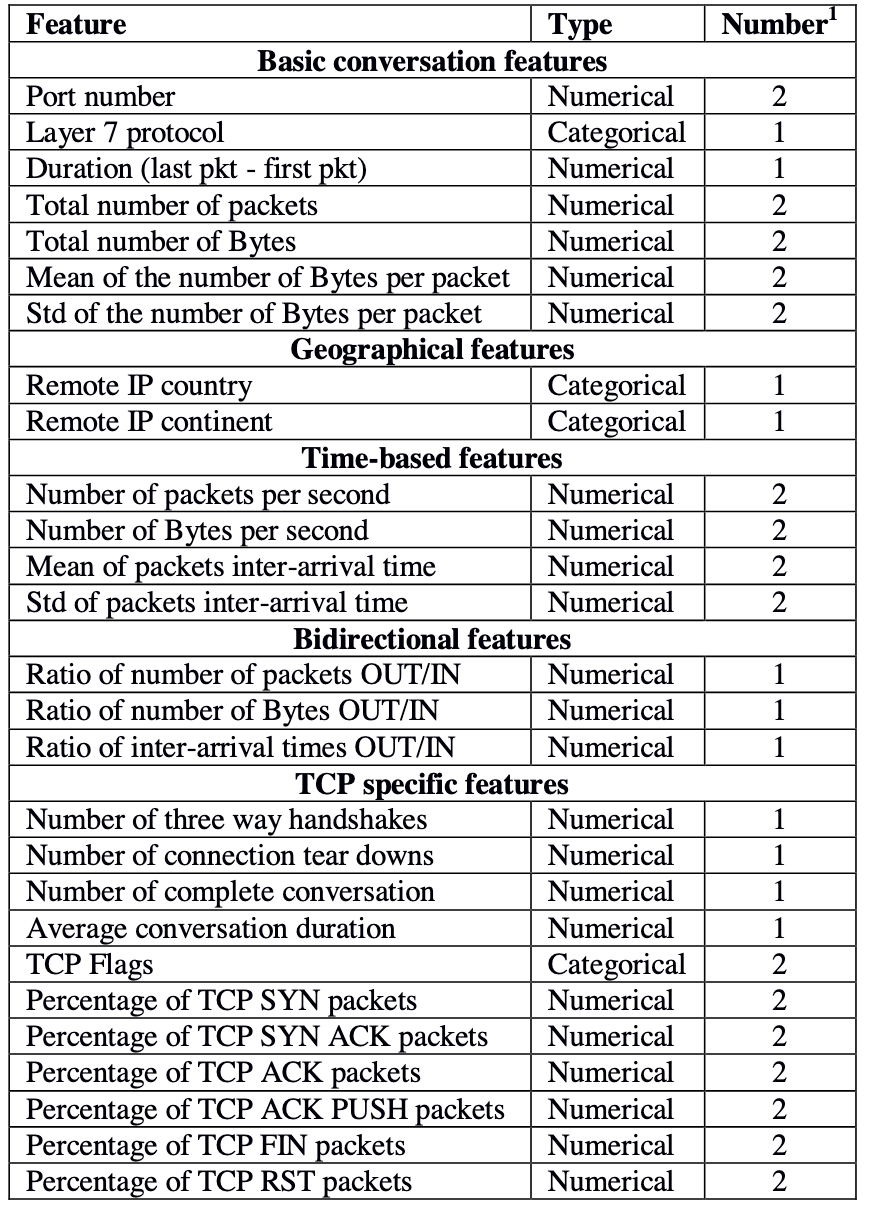
\includegraphics[scale=0.5]{./pictures/statistic_features.png}
    \caption{TCP und UDP Informationen statistisch zusammengefasst (übernommen von \cite{DBLP:journals/ijcysa/StevanovicP16}).}
    \label{fig:stats_features}
\end{figure}

\begin{figure}[h!]
    \centering
    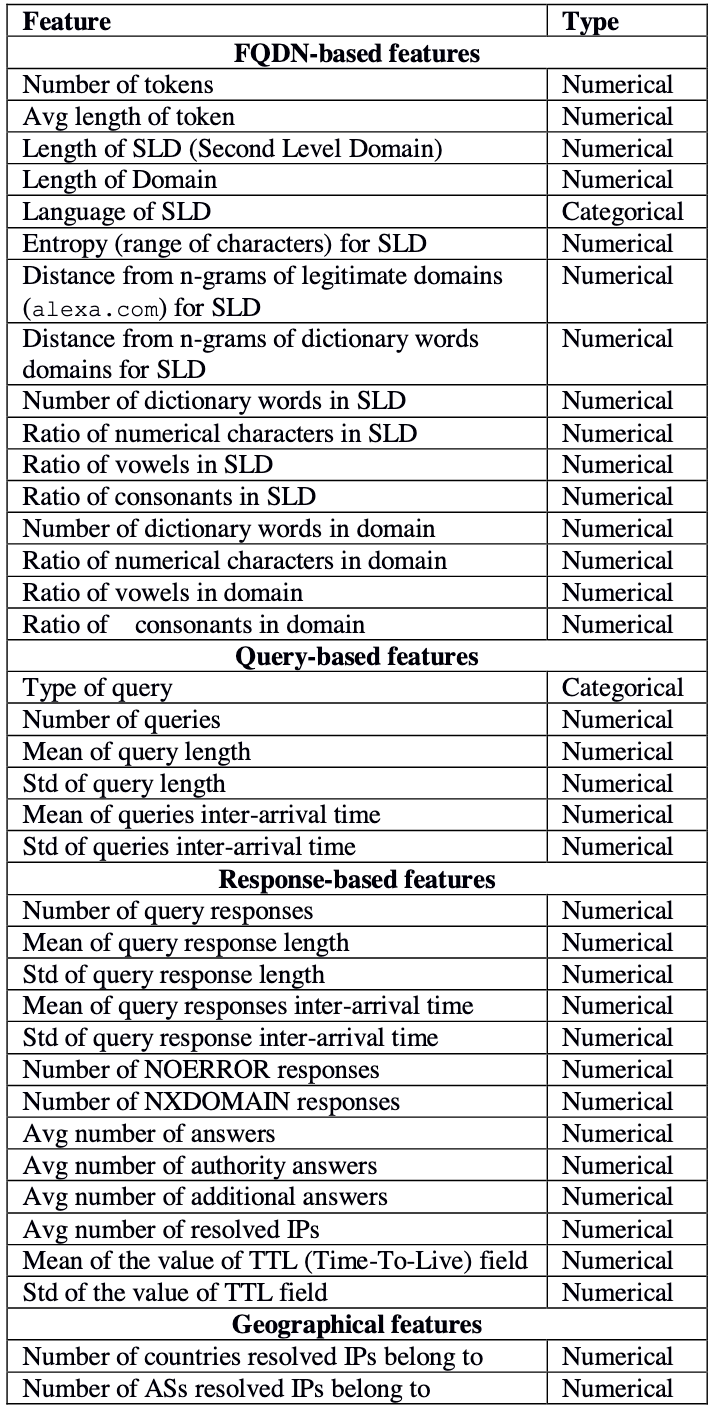
\includegraphics[scale=0.5]{./pictures/statistic_dns.png}
    \caption{DNS Informationen statistisch zusammengefasst (übernommen von \cite{DBLP:journals/ijcysa/StevanovicP16}).}
    \label{fig:stats_dns}
\end{figure}

Bei der DNS Analyse werden Fully Qualified Domain Names (FQDN) beobachtet und für jeden FQDN, statistische Eigenschaften extrahiert, welche in Abbildung \ref{fig:stats_dns} aufgelistet sind. Zur 
Klassifizierung nutzt die Botnetz Erkennung einen Random Forest Classifier, um dann über eine Client Entitäten Analyse einen Report zu erstellen über infizierte Geräte. Stevanovic und Pedersen 
zeigen mit der Arbeit, dass es möglich ist, mehrere Level zur Erkennung von Botnetzen zu implementieren. Das daraus resultierende Ziel erklärt Kapitel \ref{sec:goals} ausführlicher.
Die Botnetz Erkennung nach den unterschiedlichen Methoden und Techniken über mehrere Level soll mehr Geräte vor der illegalen Verwendung von Botnetzen schützen. 

\subsection*{Angriffsmöglichkeiten zum Testen}
Um den Prozess der Botnetz Erkennung durch Fallstudien zu testen, sollen in der Dissertation verschiedene Botnetze ausgeführt werden. Dabei sollen bereits bekannte Botnetze ausgeführt werden und 
zusätzlich soll ein Botnetz implementiert werden um herauszufinden, ob das System auch neue, unbekannte Botnetze erkennt. Das Kriterium zur Auswahl sind Botnetze die den Fokus auf IoT Geräte legen. 
Kolias et al. \cite{DBLP:journals/computer/KoliasKSV17} weisen in ihrer Arbeit auf Mirai und Hajime hin, welche in der Dissertation für die Botnetzerkennung ausgeführt werden sollen.
Nach Kolias et al. besteht Mirai aus vier Komponenten, dem \textit{Bot}, dem \textit{C\&C-Server}, der \textit{loader} und der \textit{report Server}. 
Der \textit{Bot} und \textit{C\&C-Server} weichen nicht von der allgemeinen Funktionsweise ab. Der \textit{loader} übernimmt die Kommunikation mit neuen infizierten 
Geräten und verteilt ausführbare Dateien. Der \textit{report Server} verwaltet Informationen über alle Geräte im Botnetz über eine Datenbank und kommuniziert mit den neu infizierten Geräten. 
Im folgenden Ablauf operiert und kommuniziert Mirai. 
Zu Beginn scannt Mirai zufällige IP Adressen über TCP ob die Ports 23 oder 2323 zuhören. Über brute-force Angriffe sucht der bot IoT Geräte, die schlecht konfiguriert sind (z.B. Standard Login Daten die
nicht geändert wurden). Mit einer geöffneten Shell gibt der Bot Informationen über das Gerät an den report Server über einen anderen Port. Der botmaster prüft über den C\&C-Server neu ausgewählte Geräte 
und anhand des report Servers den aktuellen Status des Botnetzes. Anhand der Informationen über die Geräte kann der Botmaster entsprechende Geräte zum infizieren auswählen und über ein Infect-Befehl 
über den loader ausführen. Der loader führt auf den ausgewählten Gerät Instruktionen aus zum herunterladen der Malware Binärdatei. Dabei stellt die Malware sicher, dass keine anderen Malware Programme auf
dem Gerät ausgeführt werden und schließt sowohl Secure Shell (SSH), als auch Telnet Programme. Der neue Bot bekommt über eine Domäne vom C\&C-Server nun mögliche Angriffsbefehle. Den initialen Prozess 
der Suche nach offenen Ports führt auch Hajime durch. Hajime ist ein Peer-to-Peer Netzwerk, welches auf BitTorrent's Distributed Hash Table (DHT) aufbaut \cite{DBLP:conf/ndss/HerwigHHRL19,2017AnalyzingTP}. 
BitTorrent nutzt das Kademlia Protokoll \cite{DBLP:conf/iptps/MaymounkovM02} und zusätzlich zur direkten Peer-to-Peer Kommunikation nutzt Hajime zusätzlich das uTorrent Transport Protocol. Für weitere
technische Erläuterungen zu Hajime, analysieren \cite{DBLP:conf/ndss/HerwigHHRL19} die Phasen des Botnetzes. 

%------------------------------------------------------------------------------------------------------------
% - Laborexperiment
% - ML Modell -> Vielleicht Unsupervised Learning, passenden Algorithmus raussuchen (basierend auf den besten Erkennungsmethoden durch ML)
% - Das Paper im Auge behalten für entsprechende Begriffe
% - WAS IST DAS ZIEL? - Welche Ergebnisse will ich am Ende haben?
% - Ist ein Zusammenhang wichtig, wofür das Botnet verwendet werden soll?
% - Ich will die Erkennung von Botnetzen verbessern (Ergebnisse sollen darauf beruhen) - Wurde die Erkennung durch meine Diss verbessert?
% - Im aktuellen Stand der Forschung auf die Hauptgebiete aus der Einführung eingehen
% - Es geht hierbei nur um die Erkennung, keine Maßnahmen und keine Verteidigung (vielleicht am Ende).